\title{\centering\Large{{\textbf{Soal}}}}

\textbf{Tugas 1 (Bab 1)}
    \begin{enumerate}
        \item Pandang gerak random $p=q$ dan $m=n_1-n_2$ menyatakan perpindahan ke kanan. Setelah jumlah total langakh $N$. Hitung:
        \begin{enumerate}[(a)]
            \item Hitung rata-rata $\overline{m}$, dan $\overline{m^3}$
            \item itung nilai rata-rata $\overline{m^2}$ dan $\overline{m^4}$
        \end{enumerate}
        \item Probabilitas $W(n)$ dinyatakan dengan probabilitas $p$ terjadi nilai $n$ kali dalam kejadian $N$ dinyatakan dengan distribusi Binomial
        \begin{equation*}
            W(n)=\dfrac{N!}{n!(N-n)!}p^n(1-p)^{N-n}
        \end{equation*}
        Perimbangkan kondisi ketika $p\ll 1$ dan $n\ll N$
        \begin{enumerate}[(a)]
            \item Jika $\ln(1-p)\approx-p$. Tunjukkan $(1-p)^{N-n}$
            \item Tunjukkan bahwa $\dfrac{N!}{(N-n)!}\approx N^n$
            \item Tunjukkan bahwa $W(n)=\dfrac{\lambda^n}{(n!)e^{-\lambda}}$ dengan $\lambda=Np$ dikenal sebagai distribusi Poisson.
        \end{enumerate}
        \item Pandang distribusi Poisson
        \begin{enumerate}[(a)]
            \item Tunjukkan sifat normalisasi $\sum_{n=0}^N W_n=1$
            \item Hitung nilai $\overline{n}$
            \item Hitung nilai $\overline{(\Delta n)^2}\equiv\overline{(n-\overline{n})^2}$
        \end{enumerate}
    \end{enumerate}
\textbf{Tugas 2 (Bab 2)}
    \begin{enumerate}
        \item Sebuah partikel bermassa $m$ bergerak bebas dalam 1 dimensi. Jika posisi dan momentum masing-masing $x$ dan $p$. Diasumsikan partikel bergerak dalam sebuah kotak pada posisi $x=0$ dan $x=L$ dan energi $E$ dan $E+\delta E$. Gambarkan ruang fase partikel dalam deksripsi klasik.
        \item Pandang sebuah ensembel klasik 1 dimensi bergerak osilasi hamonik.
        \begin{enumerate}[(a)]
            \item Jika $x$ adalah perpindahan sebagai fungsi waktu $t$ yaitu $x=A\cos(\omega t+\varphi)$ dengan $\varphi$ adalah fase $(0<\psi<2\varphi)$. Probabilitas $\omega(\varphi)\,d\varphi$ pada jangkauan $\varphi$ dan $\varphi+\,d\varphi$ adalah $\omega(\varphi)\,d\varphi=(2\pi)^{-1}\,d\varphi$. Tentukan probabilitas $P(x)\,dx$ pada jangkauan $x$ dan $x+\delta x$ untuk seluruh sudut $\varphi$, nyatakan $P(x)$ dalam variabel $A$ dan $x$.
            \item Jika ensembel tersebut berada pada energi $E$ dan $E+\delta E$. Tentukan probabilitas $P(x)\,dx$ dan nyatakan $P(x)$ dalam variabel $E$ dan $x$.
            \newpage
            \begin{figure}[htp]
                \centering
                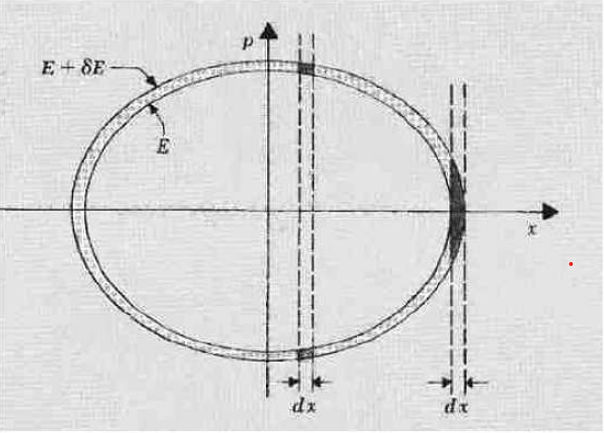
\includegraphics[width=10cm]{pic/2bab2.png}
                \caption{Deskripsi ruang fase partikel pada energi $E$ dan $E+\delta E$}
            \end{figure}
        \end{enumerate}
        \item Pandang persamaan berikut :
        \begin{equation*}
            A\,dx=B\,dy\equiv\dbar F
        \end{equation*}
        dengan $A$ dan $B$ masing-masing fungsi $X$ dan $y$
        \begin{enumerate}[(a)]
            \item Jika $\,\dbar F$ adalah diferensial eksak sehingga $F=F(x,y)$. Tunjukkan bahwa $A$ dan $B$ mengikuti 
            \begin{equation*}
                \dfrac{\partial A}{\partial y}=\dfrac{\partial B}{\partial x}
            \end{equation*}
            \item Jika $\dbar F$ adalah diferensial eksak, tunjukkan bahwa integral $\int \,\dbar F$ pada lintasan tertutup pada bidang $xy$ adalah nol.
        \end{enumerate}
    \end{enumerate}
\textbf{Tugas 3 (Bab 3)}
\begin{enumerate}
    \item Sebuah kotak dipisahkan menjadi dua bagian dengan rasio 3:1. Kotak besar mengandung 1000
    molekul gas Ne dan kotak kecil mengandung 100 molekul gas He. Sebuah lubang kecil
    dibuat antara kotak besar dan kecil dan sistem dalam kesetimbangan.
    \begin{enumerate}[(a)]
        \item Tentukan jumlah rata-rata molekul untuk setiap kotak
        \item Tentukan probabilitas dari 1000 molekul Ne dan 100 molekul Ne.
    \end{enumerate}
    \item Pandang ada sejumlah $N$ partikel dengan interaksi antar partikel diabaikan. Masing-masing partikel memiliki spin $\dfrac{1}{2}$ dan momen magnet $\mu$ dan medan magnet $H$
    \begin{enumerate}[(a)]
        \item Tentukan hubungan antara temperatur absolut $T$ dan energi total sistem $E$ menggunakan bentuk ekspresi $\beta\equiv\dfrac{\partial\ln\Omega}{\partial E}$
        \item Jika momen magnetik total adalah $M$ berkaitan dengan energi $E$. Tentukan parameter $M$ sebagai fungsi medan magnet $H$ dan temperatur $T$.
    \end{enumerate}
    \item Suatu sistem $A$ melakukan kontak termal dengan sebuah reservoir $A'$ pada temperatur $T'$. Kemudian sistem $A$ menyerap panas sejumlah $Q$ selama proses tersebut. Tunjukkan bahwa entropi $\Delta S$ pada sistem $A$ adalah $\Delta S\ge \dfrac{Q}{T'}$.
\end{enumerate}
\textbf{Tugas 4 (Bab 6)}
\begin{enumerate}
    \item Sebuah osilator harmonik 1 dimensi memiliki tingkat energi $E_n=(n+\dfrac{1}{2})\hbar\omega$ dengan $n$ adalah bilangan kuantum $(n=0, 1, 2,\dots)$ dan $\omega$ merupakan frekuesi angular. Jika osilator harmonik melakukan kontak termal dengan sebuah reservoir temperatur cukup rendah $T$ sehingga $\dfrac{kT}{\hbar\omega}\ll1$.
    \begin{enumerate}[(a)]
        \item Tentukan perbandingan probabilitas osilator harmonik pada tingkat pertama dengan tingkat dasar.
        \item Tentukan energi rata-rata dari osilator harmonik sebagai fungsi temperatur $T$ pada kondisi energi pertama dan dasar.
    \end{enumerate}
    \item Sebuah mineral minyak diletakkan pada medan magnet $H$. Setiap proton dari material memiliki spin $\dfrac{1}{2}$ dan momen magnet $\mu$. Energi proton memiliki dua keadaan yaitu $\epsilon=\mp\mu H$ dari orientasi spin. Sebuah gelombang radio diaplikasikan pada interval energi tersebut, jika frekuensi $\nu$ memenuhi kondisi Bohr $h\nu =2\nu H$. Daya yang diserap dari medan radiasi sebanding dengan perbedaan jumlah inti dari dua tingkat energi. Jika diasumsikan proton dari mineral minyak dalam keadaan kesetimbangan termal pada temperatur $T$ atau memenuhi kondisi $\nu H\ll kT$. Tentukan daya penyerapan mineral sebagai fungsi temperatur $T$.
    \item Pandang gas ideal dengan temperatur absolut $T$ didalam medan gravitasi yang uniform yang dijelaskan dengan percepatan $g$. Dengan menuliskan syarat kondisi kesetimbangan hidrostatik sebagai titik gas yang terletak diantara ketinggian $z$ dan $z+\,dz$, turunkan persamaan untuk $n(z)$ dan jumlah molekul per cm$^3$ pada ketinggian $z$. 
\end{enumerate}
\textbf{Tugas 5 (Bab 7)}
\begin{enumerate}
    \item  Sebuah gas ideal monoatomik terdiri atas $N$ partikel, masing-masing partikel bermassa $m$
    berada dalam kesetimbangan pada temperatur $T$. Gas berada dalam sebuah kotak dengan
    sisi-sisinya berukuran $L$ yang memiliki sisi bawah dan atas sejajar dengan permukaan bumi
    sehingga efek medan gravitasi $g$ pada partikel perlu diperhatikan
    \begin{enumerate}[(a)]
        \item Tentukan energi kinetik rata-rata partikel
        \item Tentukan energi potensial rata-rata partikel
    \end{enumerate}
    \item Sebuah wadah bersifat isolasi termal terdiri atas 2 bagian, masing-masing dipisahkan oleh sebuah bahan insulator. Kedua ruang berisi gas ideal memiliki kapasitas panas tetap $c_v$. Salah satu ruang memiliki jumlah $v_i$ mol dan temperatur $T_1$ dan tekanan $\bar{p}_1$ dan yang lain $v_2$ mol dan tempertaur $T_2$ dan tekanan $\bar{p}_2$. Kemudian pembatas antara 2 ruangan dihilangkan dan gas mencapai kesetimbangan
    \begin{enumerate}[(a)]
        \item Tentukan tekanan akhir
        \item Tentukan perubahan entropi $\Delta S$ jika tipe gas berbeda
    \end{enumerate} 
    \item Pandang ada sejumlah $N$ partikel dengan interaksi antar partikel diabaikan. Masing-masing
    partikel memiliki spin $\dfrac{1}{2}$ dan momen magnet $mu$ dalam medan magnet $H$. Dengan menuliskan kesetimbangan hidrostatis untuk gas yang terletak antara ketinggian $z$ dan $z+dz$, turunkan persamaan untuk $n(z)$ dan jumlah molekul per $cm^3$ pada ketinggian $z$
\end{enumerate}